%!Mode::"UTF-8"
\documentclass[12pt]{article}

% 页面设置
\usepackage{geometry}
\geometry{left=2.5cm, right=2.5cm, top=2.5cm, bottom=2.5cm}
\usepackage{graphicx}
\usepackage{ctex}
\usepackage{fontspec}
\usepackage{setspace}

% 代码设置
\usepackage{listings}
\usepackage{color}
\setmonofont{Consolas}
\definecolor{listing}{gray}{0.97}
\lstset{
	backgroundcolor=\color{listing},
	basicstyle=\footnotesize,
	numbers=left,
	numberstyle=\footnotesize,
	stepnumber=1,
	aboveskip={0.5\baselineskip},
	belowskip={0.5\baselineskip},
	columns=fullflexible,
	breaklines=true,
	breakatwhitespace=true,
	frame=single,
	basicstyle=\ttfamily,
	numberstyle=\ttfamily,
	tabsize=2
}

% 字体设置
\setmainfont{Times New Roman}
\setCJKmainfont{SimSun}
\setCJKsansfont{SimHei}
\usepackage[version=4]{mhchem}
\usepackage{mathtools}
\usepackage{diffcoeff}

% 表格设置
\usepackage{makecell}
\newcommand{\addcell}[2][4]{\makecell{\zihao{#1}\textsf{#2}}}
\usepackage{titlesec}
\usepackage{booktabs}
\usepackage{tabularx}

% 设置图注、表注
\usepackage{caption}
\usepackage{bicaption}
\captionsetup{labelsep=quad, font={small, bf}, skip=2pt}
\DeclareCaptionOption{english}[]{
    \renewcommand\figurename{Fig.}
    \renewcommand\tablename{Table}
}
\captionsetup[bi-second]{english}

% 设置页眉
\usepackage{fancyhdr}
\pagestyle{fancy}
\fancypagestyle{preContent}{
    \fancyhead[L]{\zihao{-5} 物理化学实验}
    \fancyhead[C]{\zihao{-5} 实验九\ \ 稀溶液法测定极性分子的偶极矩}
    \fancyhead[R]{\zihao{-5} 1800011828\ 王宇哲}
}
\pagestyle{preContent}

%	设置首页页眉页脚
\fancypagestyle{plain}{
	\fancyhead[L]{\zihao{-5} 物理化学实验}
	\fancyhead[C]{\zihao{-5} 实验九\ \ 稀溶液法测定极性分子的偶极矩}
	\fancyhead[R]{\zihao{-5} 1800011828\ 王宇哲}
	\cfoot{}
}

% 设置标题格式
\titleformat*{\section}{\zihao{4}\sffamily}
\titleformat*{\subsection}{\zihao{-4}\sffamily}
\titleformat*{\subsubsection}{\zihao{-4}\sffamily}
\titlespacing*{\section}{0pt}{10pt}{10pt}
\titlespacing*{\subsection}{0pt}{10pt}{5pt}
\titlespacing*{\subsubsection}{0pt}{10pt}{5pt}

% 设置引用格式
\usepackage[super,round,comma,compress]{natbib}

\usepackage{amsmath}
\usepackage{amssymb}

%设置封面
\begin{document}
    % 标题页
    \begin{titlepage}
    	% 页眉
    	\thispagestyle{plain}
        % 图片
        \begin{figure}[h]
            \centering
            \includegraphics{pku.png}
        \end{figure}
        \vspace{24pt}
        % 标题
        \centerline{\zihao{-0} \textsf{物理化学实验报告}}
        \vspace{40pt} % 空行
        \begin{center}
            \begin{tabular}{cp{11.5 cm}}
                % 题目
                \addcell[2]{题目:\ } & \addcell[2]{稀溶液法测定极性分子的偶极矩} \\
                \cline{2-2}
            \end{tabular}
        \end{center}
        \vspace{20pt} % 空行
        \begin{center}
            \doublespacing
            \begin{tabular}{cp{5cm}}
                % 姓名
                \addcell{姓\phantom{空格}名:\ } & \addcell{王宇哲} \\
                \cline{2-2}
                % 学号
                \addcell{学\phantom{空格}号:\ } & \addcell{1800011828}\\
                \cline{2-2}
                % 组别
                \addcell{组\phantom{空格}别:\ } & \addcell{11组3号} \\
                \cline{2-2}
                % 实验日期
                \addcell{实验日期:\ } & \addcell{2020.12.30}\\
                \cline{2-2}
                % 室温
                \addcell{室\phantom{空格}温:\ } & \addcell{289.75\ K}\\
                \cline{2-2}
                % 大气压强
                \addcell{大气压强:\ } & \addcell{103.43\ kPa}\\
                \cline{2-2}
            \end{tabular}
            \begin{tabular*}{\textwidth}{c}
                \\ % 这是空行
                \\ % 这是空行
                \\ % 这是空行
                \\ % 这是空行
                \hline % 分割线
            \end{tabular*}
        \end{center}
        % 摘要
        \textsf{摘\ \ 要}\ \ 本实验通过稀溶液法测定正丁醇的偶极矩,通过测定不同浓度正丁醇-环己烷溶液密度、介电常数和正丁醇折射率,计算正丁醇摩尔极化度$\overline{P}^{\infty}_{2}=(81.3\pm 0.5)\ \ {\rm mL\cdot mol^{-1}}$,最终计算正丁醇偶极矩$\mu=(1.68\pm 0.01)\ \ {\rm D}$,与文献值的相对偏差$\xi=1.2\%$,并讨论了温度变化对实验结果的影响。
        \\
        \\
        % 关键字
        \textsf{关键词}\ \ 偶极矩;电子极化;介电常数;正丁醇-环己烷体系
    \end{titlepage}

    \section{引言}
	略
               
\vbox{}        
    \section{实验部分}
    	\subsection{仪器和试剂}
    	正丁醇(AR),环己烷(AR),丙酮(AR),乙醇(AR),去离子水。\par 
    	PCM-1A型精密电容测量仪,电容池,玻璃注射器,洗耳球,$\rm 50\ \ mL$磨口锥形瓶,滴管,吸量管,比重管,DE45型数字密度计,烧杯($\rm 200\ \ mL$两个),电子天平,阿贝折射仪,循环水真空泵。
     
\vbox{}
    	 \subsection{实验内容\citealp{physchemlab}}
			\subsubsection{溶液的配制}
			取$2$个磨口锥形瓶用于盛正丁醇和环己烷,另外$5$个用于配制摩尔分数分别为$0.05$、$0.08$、$0.10$、$0.12$、$0.15$的正丁醇/环己烷溶液各$\rm 15\ \ mL$。根据预定摩尔分数算出每份溶液所需的正丁醇和环己烷的体积,按计算结果用移液管从锥形瓶中移取环己烷和正丁醇,用电子天平准确称出空锥形瓶的质量$m_{0}$、加入正丁醇后质量$m_{1}$、加入环己烷后质量$m_{2}$,摇晃均匀,算出各自的摩尔分数,塞好盖子防止挥发。
		
			\subsubsection{介电常数的测定}
			打开精密电容测定仪电源,预热$\sim 20\ \ {\rm min}$。拔下电容池与测定仪的连接插头使电路断开,按下“校零”按钮使仪表读数为$000.00$。保证电容池内干净干燥,将插头重新插入仪器面板插座内,记录测定仪示数,即为该电容池以空气为介质的电容值$C^{\prime}_{\rm E}$(E即Empty)。\par 
			取下电容池上盖,放在专用支架上,用干燥的滴管吸取环己烷$\sim 2\ \ {\rm mL}$加入电容池内至满池。轻放电容池上盖盖好电容池,读取电容值$C^{\prime}_{S}=C^{\prime}_{\rm Cy}$(S即Sample)。\par 
			用胶头滴管吸出电容池腔中的液体,再用吹风机冷风吹干电容池腔和上盖,使电容池内干净干燥,盖上池盖,记录$C^{\prime}_{\rm E}$,重新装样再测电容值$C^{\prime}_{S}=C^{\prime}_{\rm Cy}$,直到两次测定数据差不大于$\rm 0.01\ \ pF$。\par 
			用同样的方法测定各溶液的电容$C^{\prime}_{\rm S}$,同样要求两次测定数据差不大于$\rm 0.01\ \ pF$。
			
			\subsubsection{密度的测定}
			用注射器吸取$\sim \rm 7\ \ mL$环己烷,向DE45型数字密度计样品池中注入$\sim 5\ \ {\rm mL}$环己烷,排出气泡,按下“MEASURE”键测量环己烷密度;记录读数后再向样品池中注入$\sim 1\ \ {\rm mL}$环己烷,重复测量过程,共进行$3$次密度测量。测量完毕后排空样品池,长按“PUMP”键吹气除去样品池中剩余溶液。用同样的方法测定其余5种溶液及正丁醇的密度。\par 
			练习使用比重管,向比重管中注入去离子水,定容至刻度线,小心擦干比重管外壁,用电子天平称量比重管质量。倒干比重管中去离子水,重复上述测量过程,直至两次测定比重管质量差$<2\ \ {\rm mg}$。用同样的方法测定装入正丁醇的比重管质量,只测一次。用乙醇洗涤比重管,在循环水泵上抽干,用电子天平称量空比重管的质量。根据实验数据计算正丁醇的密度。
			\subsubsection{折射率的测定}
			利用阿贝折射仪测定正丁醇的折射率。


 \section{数据与结果}
 \subsection{实验数据记录及处理}
\subsubsection{溶液的配制及$\chi_{\rm BuOH}$的计算} 
 配制$5$个不同浓度的正丁醇-环己烷溶液,分别用电子天平准确称出空锥形瓶的质量$m_{0}$、加入正丁醇后质量$m_{1}$、加入环己烷后质量$m_{2}$,计算加入正丁醇的质量
 $$
 m_{\rm BuOH}=m_{1}-m_{0}
 $$
 加入环己烷的质量
 $$
 m_{\rm Cy}=m_{2}-m_{1}
 $$
 则正丁醇的摩尔分数$\chi_{\rm BuOH}$可由下式求算:
 $$
 \chi_{\rm BuOH}=\frac{m_{\rm BuOH} / M_{\rm BuOH}}{m_{\rm Cy} / M_{\rm Cy}+m_{\rm BuOH} / M_{\rm BuOH}}
 $$
 以溶液1为例,计算
 $$
 m_{\rm BuOH}=m_{1}-m_{0}=49.142\ \ {\rm g}-48.639\ \ {\rm g}=0.503\ \ {\rm g}
 $$
 $$
 m_{\rm Cy}=m_{2}-m_{1}=60.269\ \ {\rm g}-49.142\ \ {\rm g}=11.127\ \ {\rm g}
 $$
 故
 $$
 \chi_{\rm BuOH}=\frac{m_{\rm BuOH} / M_{\rm BuOH}}{m_{\rm Cy} / M_{\rm Cy}+m_{\rm BuOH} / M_{\rm BuOH}}=\frac{0.503 / 74.121}{0.503 / 74.121+ 11.127/ 84.16}=0.0488
 $$
 配制5个不同浓度的正丁醇溶液的相关实验数据及$\chi_{\rm BuOH}$的计算值如\textbf{表1}所示。
\begin{table}[h]
	\centering
	\zihao{5}
	\bicaption{正丁醇溶液配制相关实验数据及$\chi_{\rm BuOH}$计算值}{Correlative experimental data of $\rm n-BuOH$ solution preparation and $\chi_{\rm BuOH}$ calculated value}
	\begin{tabular}{ccccccccc}
		\toprule
		编号 & $V_{\rm BuOH}/{\rm mL}$ & $V_{\rm Cy}/{\rm mL}$ & $m_{0}/{\rm g}$ & $m_{1}/{\rm g}$ & $m_{2}/{\rm g}$ & $m_{\rm BuOH}/{\rm g}$ & $m_{\rm Cy}/{\rm g}$ & $\chi_{\rm BuOH}$ \\
		\midrule
		1 & 0.64 & 1.36 & 48.639 & 49.142 & 60.269 & 0.503 & 11.127 & 0.0488 \\
		2 & 1.03 & 0.97 & 46.923 & 47.711 & 58.558 & 0.788 & 10.847 & 0.0762 \\
		3 & 1.29 & 0.71 & 37.675 & 38.679 & 49.326 & 1.004 & 10.647 & 0.0967 \\
		4 & 1.55 & 0.45 & 64.419 & 65.614 & 76.081 & 1.195 & 10.467 & 0.1148 \\
		5 & 1.95 & 0.05 & 43.249 & 44.793 & 54.860 & 1.544 & 10.067 & 0.1483 \\
		\bottomrule
	\end{tabular}
\end{table}
\par


\subsubsection{介电常数的测定}
用精密电容测量仪测量环己烷及$5$个不同浓度的正丁醇溶液对应的电容值,直至相邻两次测定数据差不大于$0.01\ \ {\rm pF}$,分别计算电容池以空气为介质的电容值的平均值$\overline{C^{\prime}_{\rm E}}$及以待测溶液为介质的电容值的平均值$\overline{C^{\prime}_{\rm S}}$,相关数据如\textbf{表2}所示。

\begin{table}[h]
	\centering
	\zihao{5}
	\bicaption{各溶液电容值测定相关实验数据}{Correlative experimental data of determination of capacitance of each solution}
	\begin{tabular}{ccccccccc}
		\toprule
		编号 & $C^{\prime}_{\rm E1}/{\rm pF}$ & $C^{\prime}_{\rm S1}/{\rm pF}$ & $C^{\prime}_{\rm E2}/{\rm pF}$ & $C^{\prime}_{\rm S2}/{\rm pF}$ & $C^{\prime}_{\rm E3}/{\rm pF}$ & $C^{\prime}_{\rm S3}/{\rm pF}$ & $\overline{C^{\prime}_{\rm E}}/{\rm pF}$ & $\overline{C^{\prime}_{\rm S}}/{\rm pF}$ \\
		\midrule
		Cy & 4.38 & 7.02 & 4.29 & 6.91 & 4.30 & 6.92 & 4.30 & 6.92 \\
		1  & 4.30 & 7.07 & 4.30 & 7.07 &      &      & 4.30 & 7.07 \\
		2  & 4.30 & 7.21 & 4.30 & 7.21 &      &      & 4.30 & 7.21 \\
		3  & 4.30 & 7.33 & 4.29 & 7.33 &      &      & 4.30 & 7.33 \\
		4  & 4.29 & 7.49 & 4.29 & 7.45 & 4.29 & 7.45 & 4.29 & 7.45 \\
		5  & 4.29 & 7.77 & 4.30 & 7.78 &      &      & 4.30 & 7.78 \\
		\bottomrule
	\end{tabular}
\end{table}
\par

\subsubsection{密度的测定及计算}
用DE45型数字密度计准确测定各溶液的密度,计算溶液密度平行测定值的平均值$\overline{\rho}$,结果如\textbf{表3}所示。
\begin{table}[h]
	\centering
	\zihao{5}
	\bicaption{各溶液密度测定相关实验数据}{Correlative experimental data of determination of density of each solution}
	\begin{tabular}{ccccc}
		\toprule
		编号 & $\rho_{1}/{\rm g\cdot mL^{-1}}$ & $\rho_{2}/{\rm g\cdot mL^{-1}}$ & $\rho_{3}/{\rm g\cdot mL^{-1}}$ & $\overline{\rho}/{\rm g\cdot mL^{-1}}$ \\
		\midrule
		Cy   & 0.77859 & 0.77859 & 0.77859 & 0.77859 \\
		1    & 0.77889 & 0.77890 & 0.77890 & 0.77890 \\
		2    & 0.77930 & 0.77930 & 0.77930 & 0.77930 \\
		3    & 0.77964 & 0.77960 & 0.77962 & 0.77962 \\
		4    & 0.77994 & 0.77994 & 0.77994 & 0.77994 \\
		5    & 0.78057 & 0.78055 & 0.78056 & 0.78056 \\
		BuOH & 0.80964 & 0.80964 & 0.80964 & 0.80964 \\
		\bottomrule
	\end{tabular}
\end{table}
\par

练习使用比重管测定液体密度,相关数据如\textbf{表4}所示,其中$M_{1}$、$M_{2}$为加入去离子水后比重管质量的两次测量结果,$M_{\rm BuOH}$为加入$\rm BuOH$后比重管质量的测量结果、$M_{0}$为空比重管质量的测量结果。
\begin{table}[h]
	\centering
	\zihao{5}
	\bicaption{使用比重管测定液体密度相关实验数据}{Correlative data of determination of liquid density using pycnometer}
	\begin{tabular}{cccc}
		\toprule
		$M_{1}/{\rm g}$ & $M_{2}/{\rm g}$ & $M_{\rm BuOH}/{\rm g}$ & $M_{0}/{\rm g}$ \\
		\midrule
		30.105 & 30.107 & 29.238 & 25.400 \\
		\bottomrule
	\end{tabular}
\end{table}
\par
故两次测量时水的质量
$$m_{1}=M_{1}-M_{0}=4.705\ \ {\rm g}$$
$$m_{2}=M_{2}-M_{0}=4.707\ \ {\rm g}$$
水的质量的平均值$$m=\frac{m_{1}+m_{2}}{2}=4.706\ \ {\rm g}$$
测量正丁醇密度时,正丁醇的质量
$$m_{\rm BuOH}=M_{\rm BuOH}-M_{0}=3.838\ \ {\rm g}$$
查手册知室温$T=18.9\ \ {\rm ^{\circ}C}$下水的密度$\rho=0.99845\ \ {\rm g\cdot mL^{-1}}$,故计算正丁醇的密度
$$
\rho_{\rm BuOH}=\frac{m_{\rm BuOH}}{m}\rho=\frac{3.838\times 0.99845}{4.706}=0.81429\ \ {\rm g\cdot mL^{-1}}
$$


\subsubsection{折射率的测定}
使用阿贝折射仪测定正丁醇的折射率
$$
n_{\rm BuOH}=1.4011
$$
并记录阿贝折射仪上温度计示数为$12.7\ \ {\rm ^{\circ}C}$。

\vbox{}


 \subsection{数据处理结果与分析}
 \subsubsection{介电常数的计算}
环己烷的介电常数$\varepsilon_{\rm Cy}$与温度$T$的关系为
$$
\varepsilon_{\rm Cy}=2.023-0.0016\ \ (\frac{T}{\rm K}-293)
$$
室温$T=289.15\ \ {\rm K}$,故计算
$$
\varepsilon_{\rm Cy}=2.023-0.0016\times (289.15-293)=2.029
$$
电容器的电容$C_{0}$可由下式求算:
$$
C_{0}=\frac{C^{\prime}_{\rm Cy}-C^{\prime}_{\rm E}}{\varepsilon_{\rm Cy}-1}
$$
分布电容$C_{\rm D}$(D即Distribution)可由下式求算:
$$
C_{\rm D}=C^{\prime}_{\rm E}-C_{0}
$$
则样品的介电常数$\varepsilon_{\rm S}$可由下式求算:
$$
\varepsilon_{\rm S}=\frac{C_{\rm S}}{C_{0}}
$$
其中
$$
C_{\rm S}=C^{\prime}_{\rm S}-C_{\rm D}
$$
\par 
根据\textbf{表2}数据,以$C^{\prime}_{\rm E}$、$C^{\prime}_{\rm S}$的平均值作为真实值,计算各溶液的介电常数$\varepsilon_{\rm S}$。首先根据环己烷的相关数据,计算
$$
C_{0}=\frac{C^{\prime}_{\rm Cy}-C^{\prime}_{\rm E}}{\varepsilon_{\rm Cy}-1}=\frac{6.92-4.30}{2.029-1}{\rm pF}=2.55\ \ {\rm pF}
$$
$$
C_{\rm D}=C^{\prime}_{\rm E}-C_{0}=4.30\ \ {\rm pF}-2.55\ \ {\rm pF}=1.75\ \ {\rm pF}
$$
可以近似认为分布电容$C_{\rm D}$为常数,在实验过程中保持不变,以溶液1为例,计算
$$
C_{0}=C^{\prime}_{\rm E}-C_{\rm D}=4.30\ \ {\rm pF}-1.75\ \ {\rm pF}=2.55\ \ {\rm pF}
$$
$$
C_{\rm S}=C^{\prime}_{\rm S}-C_{\rm D}=7.07\ \ {\rm pF}-1.75\ \ {\rm pF}=5.32\ \ {\rm pF}
$$
$$
\varepsilon_{\rm S}=\frac{C_{\rm S}}{C_{0}}=2.086
$$
类似地,计算各溶液的介电常数$\varepsilon_{\rm S}$,结果如\textbf{表5}所示。
\begin{table}[h]
	\centering
	\zihao{5}
	\bicaption{各溶液介电常数$\varepsilon_{\rm S}$计算数据}{Calculation data of dielectric constant $\varepsilon_{\rm S}$ of each solution}
	\begin{tabular}{ccccc}
		\toprule
		编号 & $\chi_{\rm BuOH}$ & $C_{0}/{\rm pF}$ & $C_{\rm S}/{\rm pF}$ & $\varepsilon_{\rm S}$ \\
		\midrule
		1 & 0.0488 & 2.55 & 5.32 & 2.086 \\
		2 & 0.0762 & 2.55 & 5.46 & 2.143 \\
		3 & 0.0967 & 2.55 & 5.58 & 2.190 \\
		4 & 0.1148 & 2.54 & 5.70 & 2.246 \\
		5 & 0.1483 & 2.55 & 6.03 & 2.367 \\
		\bottomrule
	\end{tabular}
\end{table}
\par

\subsubsection{正丁醇折射度$R$的计算}
正丁醇的折射度$R$可由下式求算:
$$
R=\frac{n_{\rm BuOH}^{2}-1}{n_{\rm BuOH}^{2}+2}\times \frac{M_{\rm BuOH}}{\rho_{\rm BuOH}}
$$
由3.1.4知正丁醇的折射率$n_{\rm BuOH}=1.4011$,由3.1.3知正丁醇的密度$\rho_{\rm BuOH}=0.80964\ \ {\rm g\cdot mL^{-1}}$,$M_{\rm BuOH}=74.12\ \ {\rm g\cdot mol^{-1}}$,代入公式计算得
$$
R=\frac{n_{\rm BuOH}^{2}-1}{n_{\rm BuOH}^{2}+2}\times \frac{M_{\rm BuOH}}{\rho_{\rm BuOH}}=\frac{1.4011^{2}-1}{1.4011^{2}+2}\times \frac{74.12\ \ {\rm g\cdot mol^{-1}}}{0.80964\ \ {\rm g\cdot mL^{-1}}}=22.247\ \ {\rm mL\cdot mol^{-1}}
$$
\subsubsection{$\varepsilon_{\rm S}-\chi_{\rm BuOH}$图}
根据\textbf{表5}数据,作出$\varepsilon_{\rm S}-\chi_{\rm BuOH}$关系的散点图,并用python SciPy lingress进行线性拟合,作出拟合直线,如\textbf{图1}所示。

\begin{figure}[h]
	\centering
	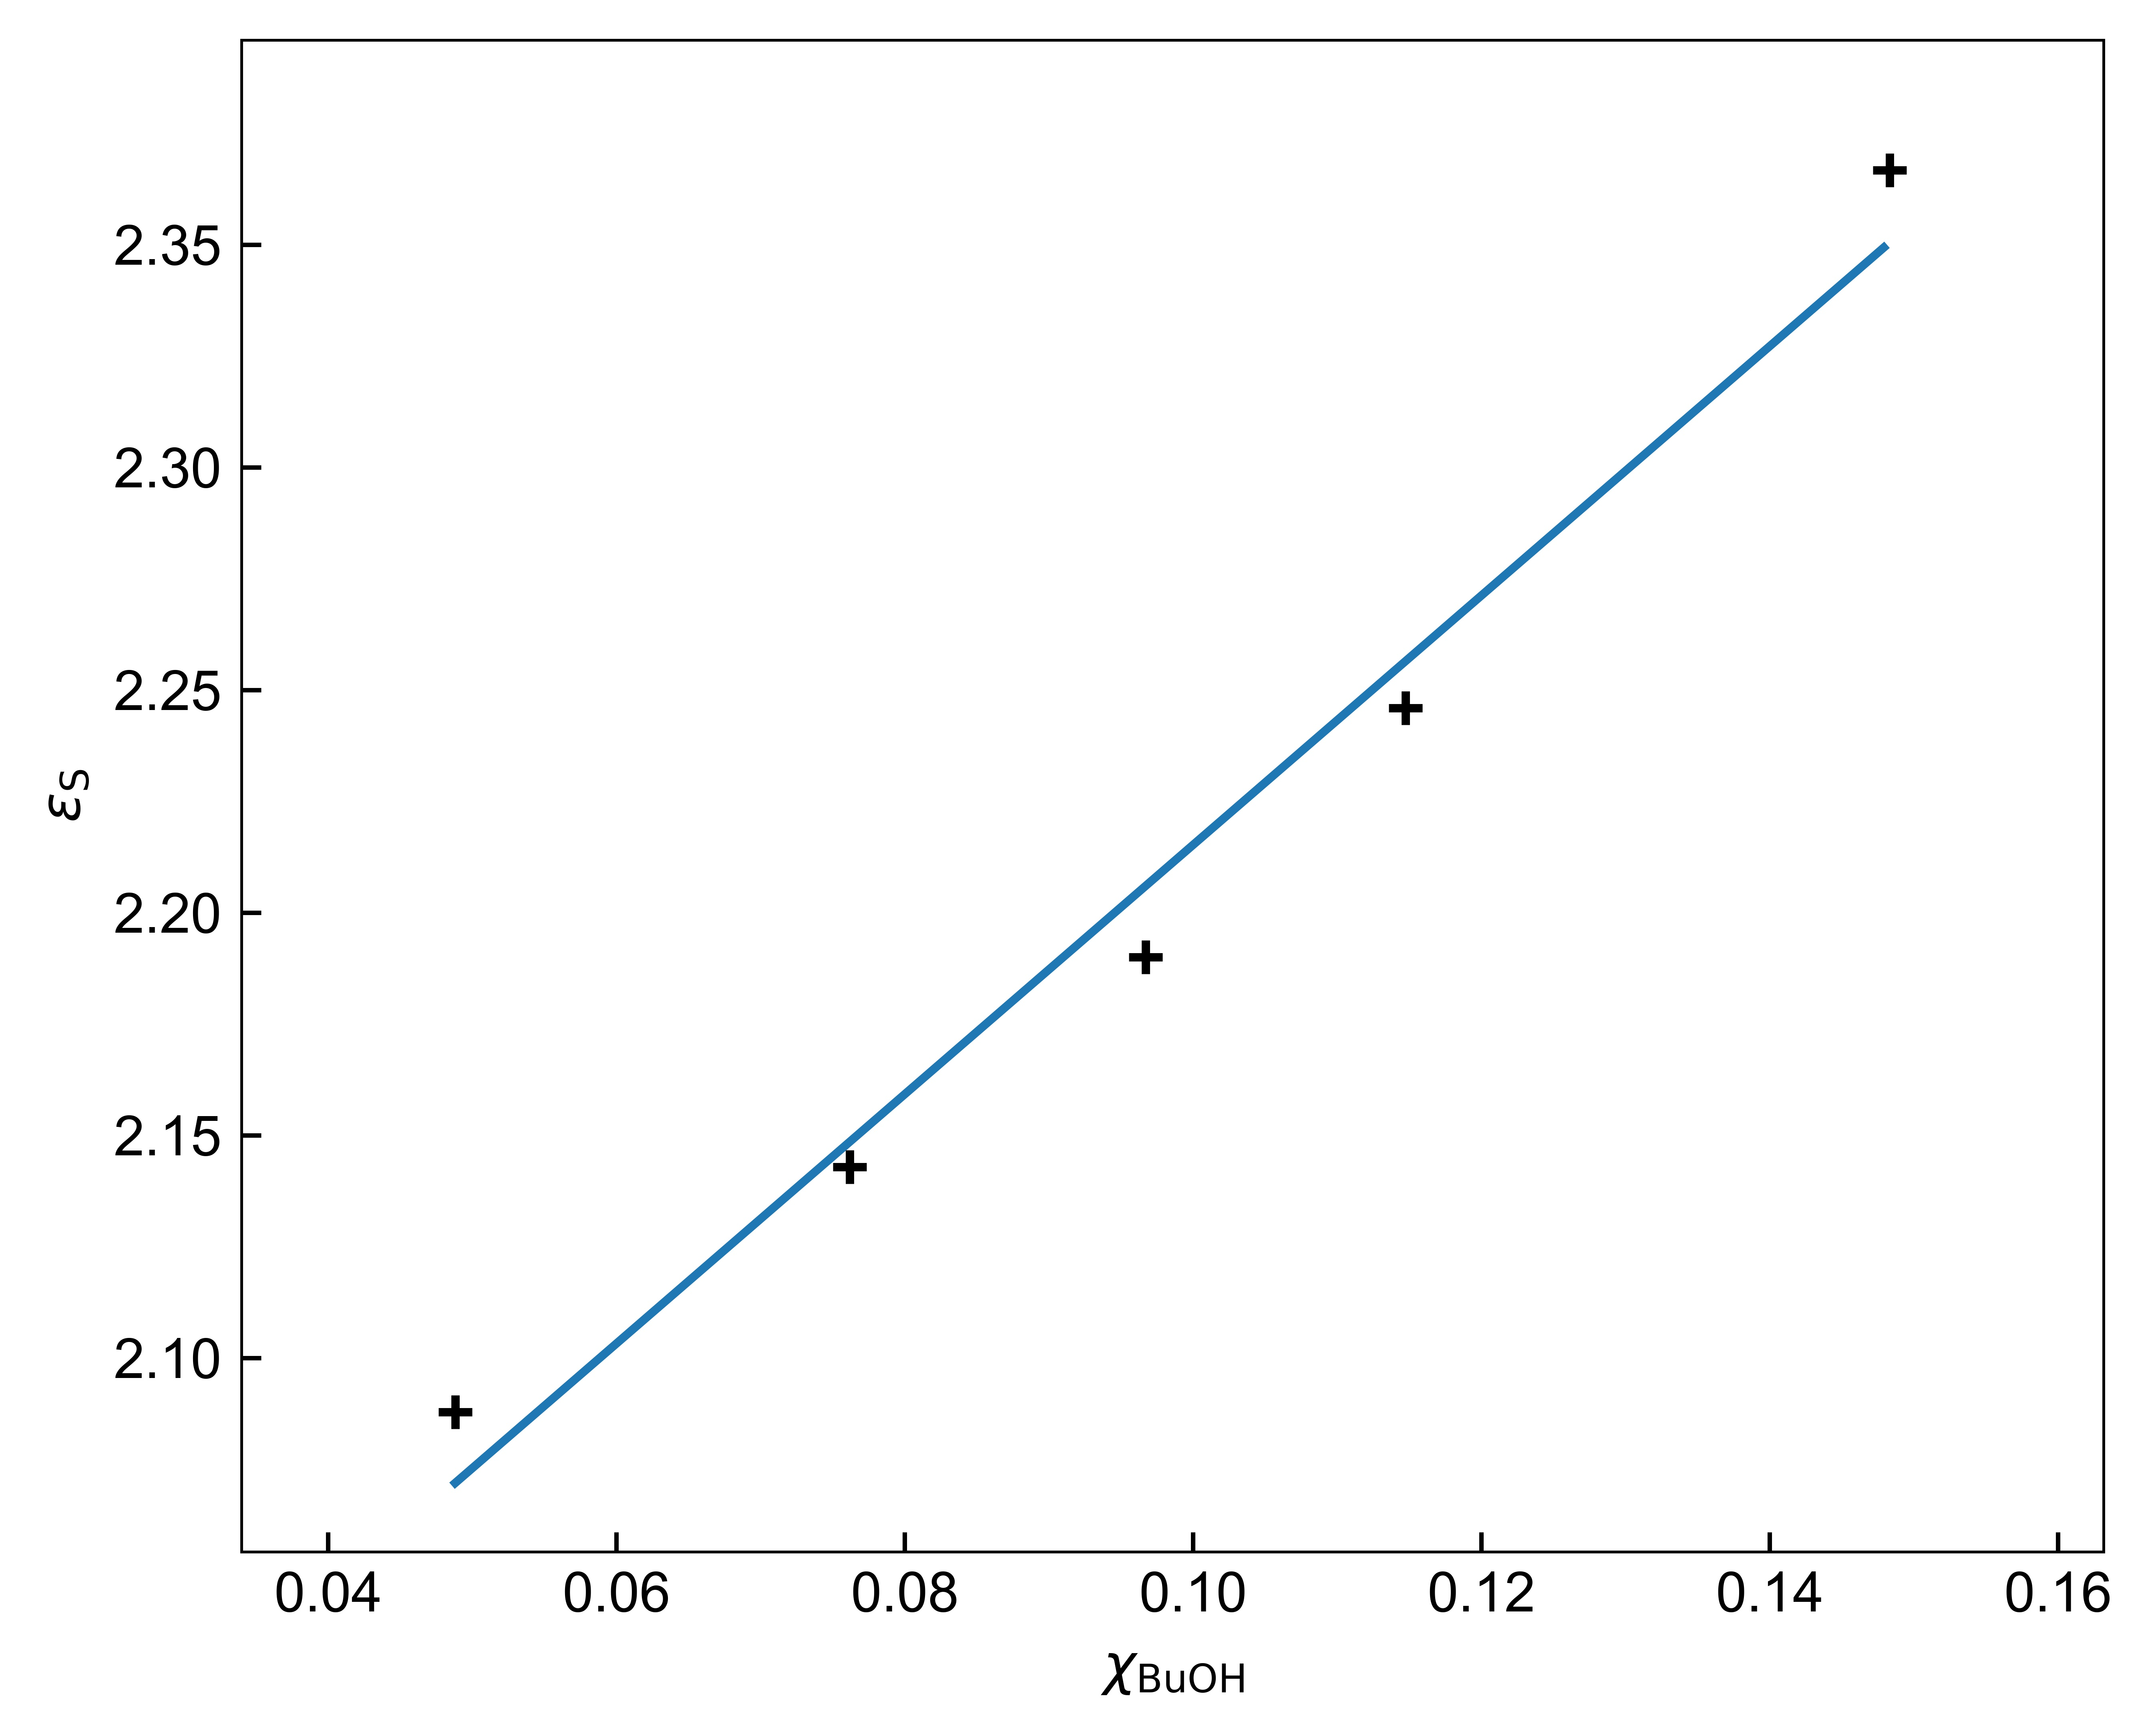
\includegraphics[width=0.65\textwidth]{1.jpg}
	\bicaption{$\varepsilon_{\rm S}-\chi_{\rm BuOH}$关系图及线性拟合}{$\varepsilon_{\rm S}-\chi_{\rm BuOH}$ diagram and linear fit}
\end{figure}
\par

拟合直线的方程为
$$
\varepsilon_{\rm S}=(2.8\pm 0.2)\chi_{\rm BuOH}+(1.94\pm 0.02),\  \ R=0.9898
$$
故直线截距
$$\varepsilon_{1}=1.94\pm 0.02$$
直线斜率
$$a=2.8\pm 0.2$$

\subsubsection{$\overline{\rho}-\chi_{\rm BuOH}$图}
根据\textbf{表1}及\textbf{表3}数据,作出$\overline{\rho}-\chi_{\rm BuOH}$关系的散点图,并用python SciPy lingress进行线性拟合,作出拟合直线,如\textbf{图2}所示。

\begin{figure}[h]
	\centering
	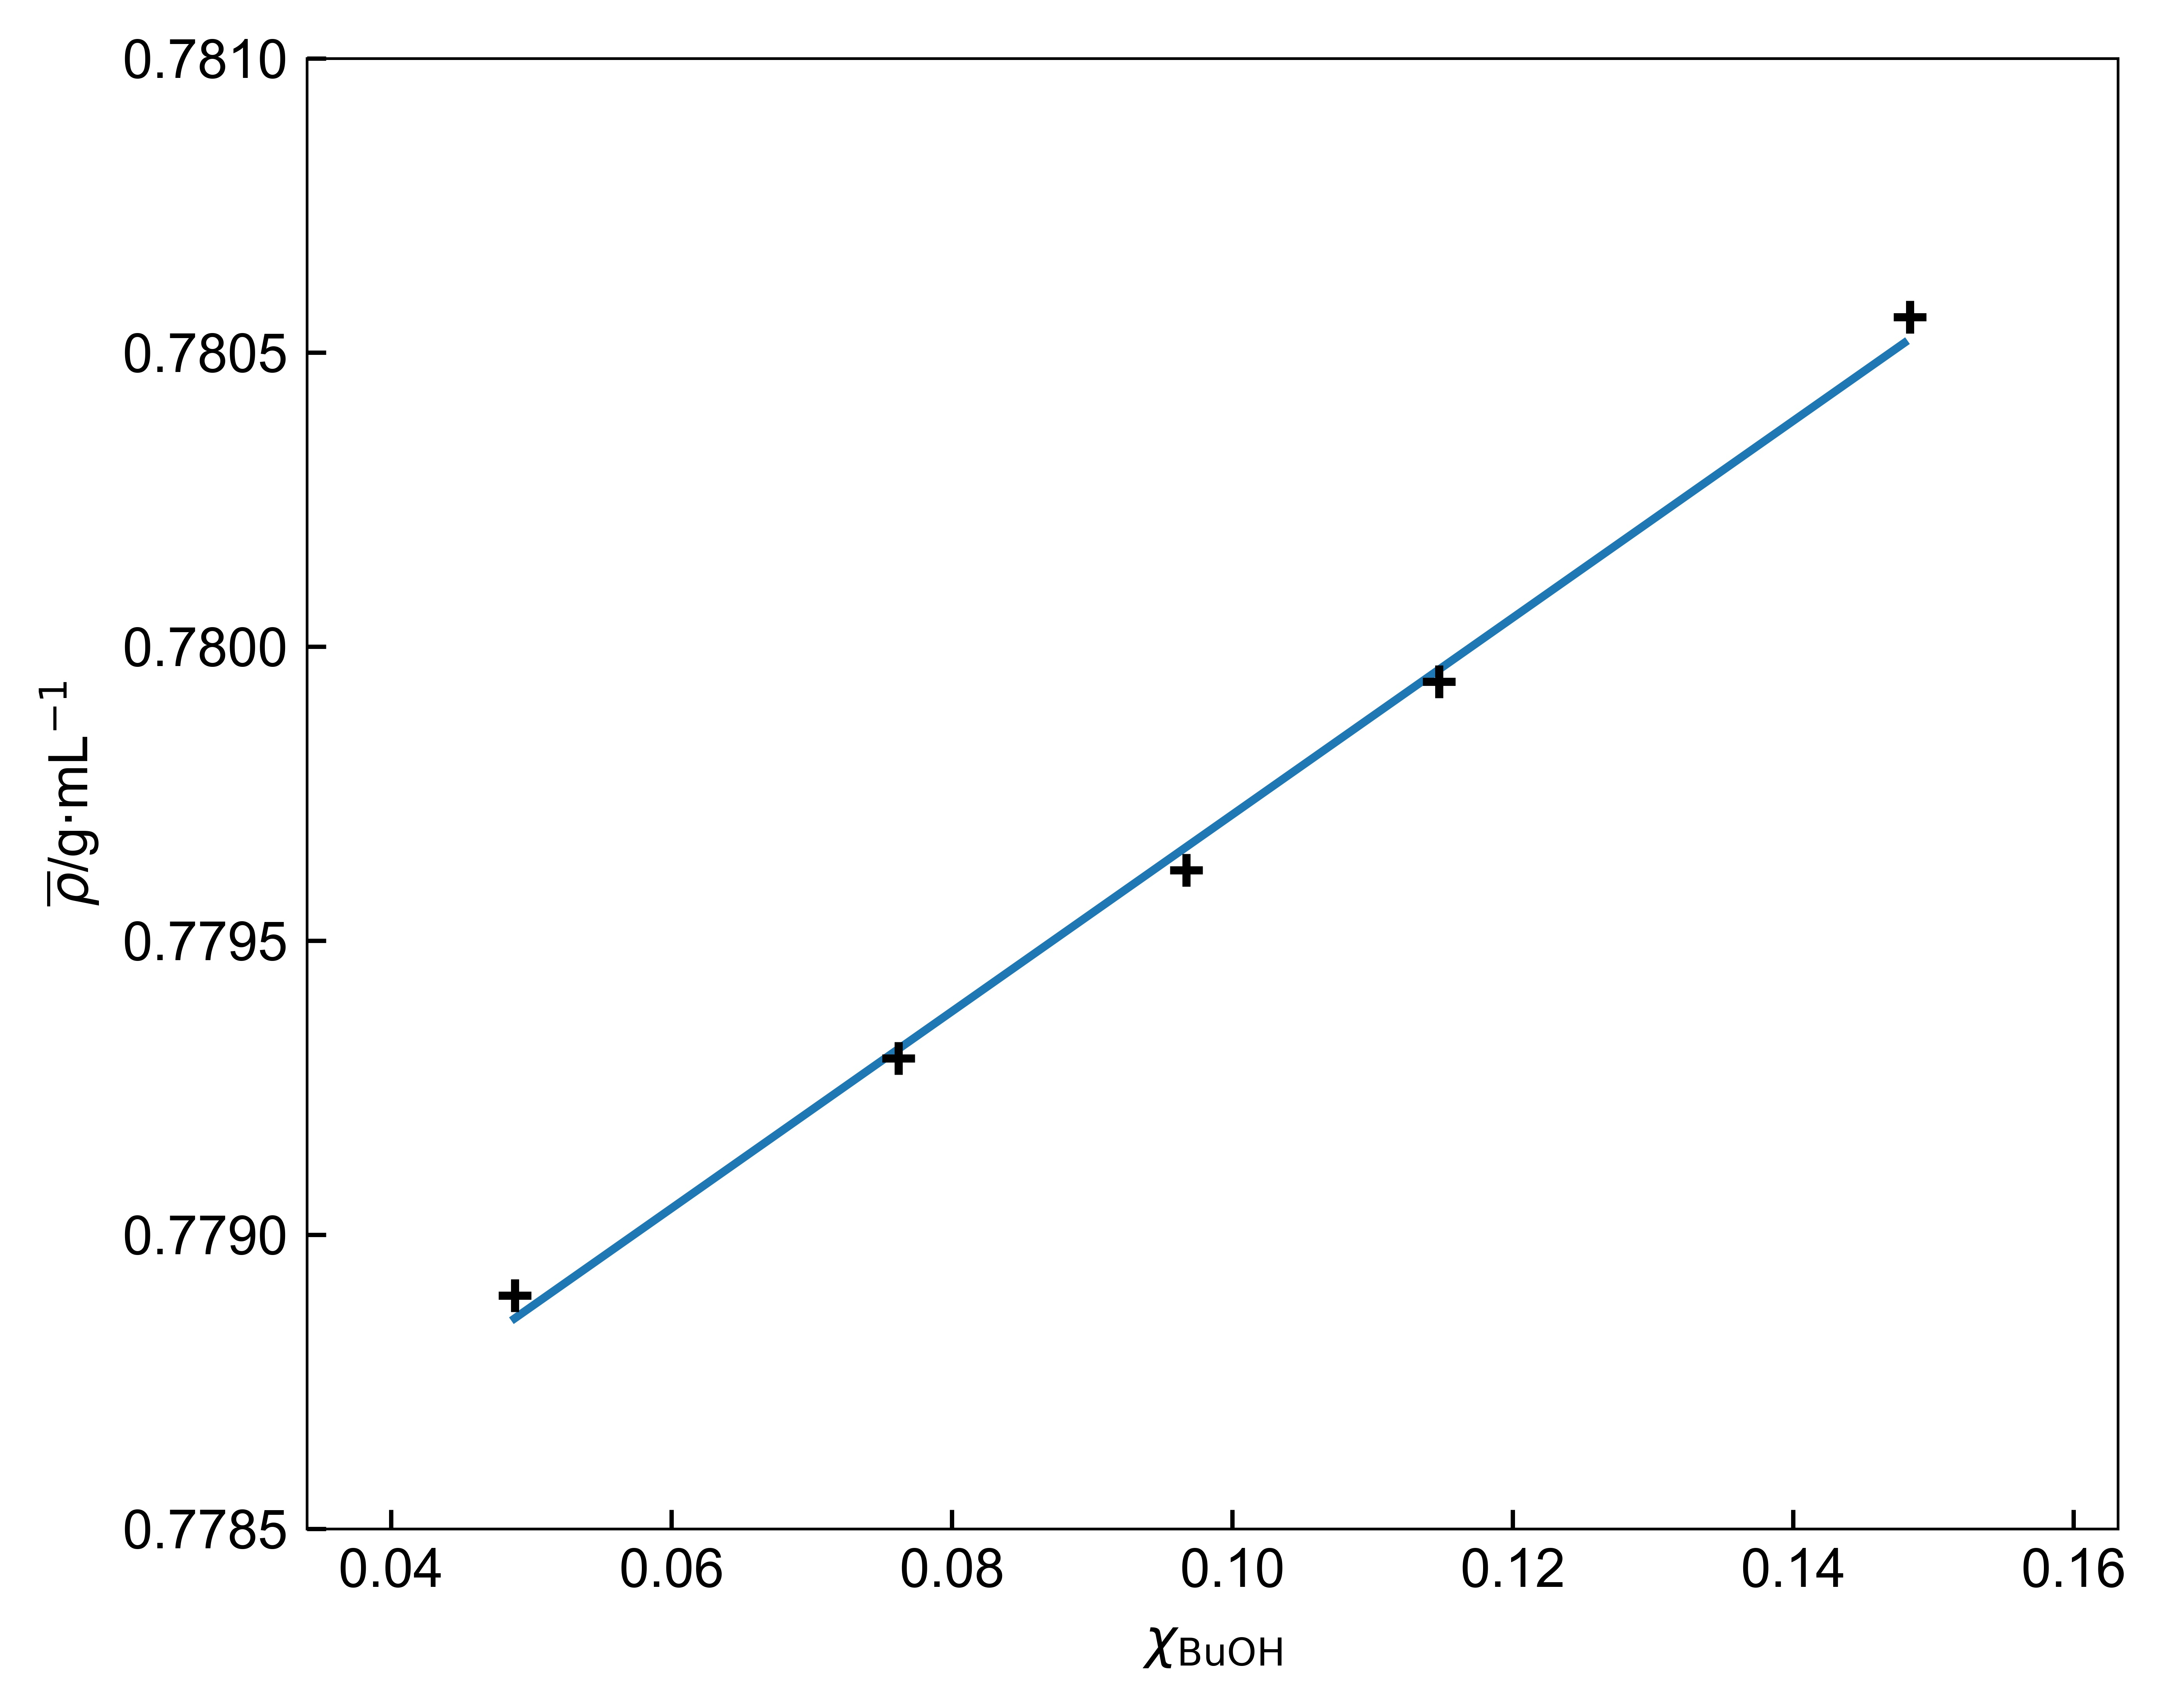
\includegraphics[width=0.65\textwidth]{2.jpg}
	\bicaption{$\overline{\rho}-\chi_{\rm BuOH}$关系图及线性拟合}{$\overline{\rho}-\chi_{\rm BuOH}$ diagram and linear fit}
\end{figure}
\par

拟合直线的方程为
$$
\overline{\rho}/{\rm g\cdot mL^{-1}}=(0.0167\pm 0.0005)\chi_{\rm BuOH}+(0.77804\pm 0.00005),\  \ R=0.9984
$$
故直线截距
$$\rho_{1}=(0.77804\pm 0.00005)\ \ {\rm g\cdot mL^{-1}}$$
直线斜率
$$b=(0.0167\pm 0.0005)\ \ {\rm g\cdot mL^{-1}}$$

\subsubsection{$\overline{P}^{\infty}_{2}$的计算}
正丁醇的摩尔极化度$\overline{P}^{\infty}_{2}$可由下式近似求算:
$$
\overline{P}^{\infty}_{2}=A(M_{2}-bB)+aC
$$
其中,
$$
A=\frac{\varepsilon_{1}-1}{\varepsilon_{1}+2}\times \frac{1}{\rho_{1}}
$$
$$
B=\frac{M_{1}}{\rho_{1}}
$$
$$
C=\frac{3M_{1}}{(\varepsilon_{1}+2)^{2}\rho_{1}}
$$
由3.2.3和3.2.4知$\varepsilon_{1}=1.94\pm 0.02$,$a=2.8\pm 0.2$,$\rho_{1}=(0.77804\pm 0.00005)\ \ {\rm g\cdot mL^{-1}}$,$b=(0.0167\pm 0.0005)\ \ {\rm g\cdot mL^{-1}}$,代入计算得
$$
A=\frac{2.10-1}{2.10+2}\times \frac{1}{0.77804\ \ {\rm g\cdot mL^{-1}}}=0.307\ \ {\rm mL\cdot mol^{-1}}
$$
$$
B=\frac{84.16\ \ {\rm g\cdot mol^{-1}}}{0.77804\ \ {\rm g\cdot mL^{-1}}}=108.169\ \ {\rm mL\cdot mol^{-1}}
$$
$$
C=\frac{3\times 84.16\ \ {\rm g\cdot mol^{-1}}}{(1.94+2)^{2}\times 0.77804\ \ {\rm g\cdot mL^{-1}}}=21.1\ \ {\rm mL\cdot mol^{-1}}
$$
故
$$
\overline{P}^{\infty}_{2}=(0.307 \times (74.12 -0.0167 \times 108.169)+2.8 \times 21.1)\ \ {\rm mL\cdot mol^{-1}} = 81.3 \ \ {\rm mL\cdot mol^{-1}} 
$$
不确定度
$$
\sigma_{A}=\sqrt{( \frac{3}{(\varepsilon_{1}+2)^{2}} \times  \frac{1}{\rho_{1}})^{2}\times \sigma^{2}_{\varepsilon_{1}}+(\frac{\varepsilon_{1}-1}{\varepsilon_{1}+2}\times \frac{1}{\rho_{1}})^{2}\sigma^{2}_{\rho_{1}}}=0.005\ \ {\rm mL\cdot mol^{-1}}
$$
$$
\sigma_{B}=B\frac{\sigma_{\rho_{1}}}{\rho_{1}}=\frac{108.2\times 0.00005}{0.77804}\ \ {\rm g\cdot mol^{-1}}=0.007\ \ {\rm  mL\cdot mol^{-1}}
$$
$$
\sigma_{C}=C\sqrt{(\frac{\sigma_{\varepsilon_{1}}}{\varepsilon_{1}+2})^{2}+(\frac{\sigma_{\rho_{1}}}{\rho_{1}})^{2}}=19.3\times \sqrt{(\frac{0.02}{1.94+2})^{2}+(\frac{0.00005}{0.77804})^{2}} \ \ {\rm mL\cdot mol^{-1}}=0.1\ \ {\rm mL\cdot mol^{-1}}
$$
故
$$
A=(0.307\pm 0.005)\ \ {\rm mL\cdot mol^{-1}}
$$
$$
B=(108.169\pm 0.007)\ \ {\rm mL\cdot mol^{-1}}
$$
$$
C=(21.1\pm 0.1)\ \ {\rm mL\cdot mol^{-1}}
$$
故$\overline{P}^{\infty}_{2}$的不确定度
$$
\sigma_{\overline{P}^{\infty}_{2}}=\sqrt{(M_{2}-bB)^{2} \sigma_{A}^{2}+A^{2} B^{2} \sigma_{b}^{2}+A^{2} b^{2} \sigma_{B}^{2}+C^{2} \sigma_{a}^{2}+a^{2} \sigma_{C}^{2}}=0.5\ \ {\rm mL\cdot mol^{-1}}
$$
故
$$
\overline{P}^{\infty}_{2}=(81.3\pm 0.5)\ \ {\rm mL\cdot mol^{-1}}
$$

\subsubsection{正丁醇偶极矩$\mu$的计算}
正丁醇的偶极矩$\mu$可由下式求算:
$$
\mu=12.81\sqrt{(\frac{\overline{P}^{\infty}_{2}}{\rm m^{3}\cdot mol^{-1}}-\frac{R}{\rm m^{3}\cdot mol^{-1}})(\frac{T}{K})}\ \ {\rm D}
$$
由3.2.5知$\overline{P}^{\infty}_{2}=(81.3\pm 0.5) \ \ {\rm mL\cdot mol^{-1}}$,由3.2.2知$R=22.247\ \ {\rm mL\cdot mol^{-1}}$,$T=289.75\ \ {\rm K}$,代入公式计算得
$$
\mu=12.81\times \sqrt{(81.3-22.247)\times 289.75}\ \ {\rm D} = 1.68\ \ {\rm D}
$$
考虑室温的波动,取$\sigma_{T}=1\ \ {\rm K}$,计算$\mu$的不确定度
$$
\sigma_{\mu}=\frac{12.81^{2}}{2} \sqrt{(\frac{T}{\mu})^{2} \sigma_{\overline{P}^{\infty}_{2}}^{2}+(\frac{\overline{P}^{\infty}_{2}-R}{\mu})^{2} \sigma_{T}^{2}}=0.01\ \ {\rm D}
$$
故
$$
\mu=(1.68\pm 0.01)\ \ {\rm D}
$$
查阅\textit{CRC Handbook of Chemistry and Physics}\citealp{crc},知正丁醇偶极矩的文献值$\mu=(1.66\pm 0.03)\ \ {\rm D}$,故实验测得正丁醇偶极矩落在参考值范围内,与参考值很好地吻合,相对误差
$$
\xi=\frac{1.68-1.66}{1.66}\times 100\%=1.2\%
$$


\vbox{}

 	\section{讨论与结论}
		\subsection{实验讨论}
 			\subsubsection{温度$T$对实验误差的影响}
 			本实验在数据处理过程中,以实验室内的大气压-温度仪示数$t=18.9\ \ {\rm ^{\circ}C}$作为实际的温度$T$,代入公式中进行计算。但在实验过程中,使用阿贝折射仪测定正丁醇的折射率时,由于阿贝折射仪放置于实验室背阴角落处,阿贝折射仪上温度示数仅为$t=12.7\ \ {\rm ^{\circ}C}$;在使用吹风机冷风吹干电容池时,明显可感觉到电吹风出风温度不同于室温,估测出风温度$t=25\ \ {\rm ^{\circ}C} $。\par 
 		温度变化对折光率和介电常数测定造成了一定的影响,查阅手册知正丁醇在$20\ \ {\rm ^{\circ}C}$下折射率$n_{\rm BuOH}=1.3993$,该温度与室温接近,依此计算实验测量的折射率与实际的折射率的相对偏差
 		$$
 		\xi_{n}=\frac{1.4011-1.3993}{1.3993}\times 100\%=0.13\%
 		$$
 		按照参考值计算正丁醇折射度
 		$$R=\frac{1.3993^{2}-1}{1.3993^{2}+2}\times \frac{74.12}{0.80964} \ \ {\rm mL\cdot mol^{-1}}=22.159\ \ {\rm mL\cdot mol^{-1}}$$
 		实验测量的折射度的相对偏差
 		$$\xi_{R}=\frac{22.247-22.159}{22.159}\times 100\%=0.40\%$$
 		而如前文所述,吹风机出风温度高于室温,电容池内温度高于$20\ \ {\rm ^{\circ}C}$,故温度对折射度$R$带来的相对偏差甚至大于上述结果。\par 
 		环己烷的介电常数根据公式
 		$$
 		\varepsilon_{\rm Cy}=2.023-0.0016\ \ (\frac{T}{\rm K}-293)
 		$$
 		得到,取实际温度为$25\ \ {\rm ^{\circ}C}$,计算
 		$$
 		\varepsilon_{\rm Cy}=2.015
 		$$
 		故室温下的计算值相对上述实际值的相对偏差
 		$$
 		\xi_{\varepsilon}=\frac{2.029-2.015}{2.015}\times 100\%=0.7\%
 		$$
 		可见温度的不同对实验过程中大量物理量的测量引入了误差,最终导致$\mu$的实验值偏离参考值。
 		\subsubsection{实验改进}
 		根据以上讨论,对实验的改进建议如下:\par 
 		控制实验室恒温,或在实验的主要仪器加装恒温水浴装置,避免不同测量仪器处温度不同,从而减少温度变化对各物理量测量的影响。
 		\subsection{实验报告勘误}
 		在撰写最初的实验报告时,由于数据誊抄错误,造成计算值出现严重错误。经张洁老师指出后,重新绘制了实验报告中的拟合曲线图,计算了各物理量的数值,得到了与文献参考值相一致的结果。本人在此对该错误深感抱歉,并对张老师表示由衷感谢。
 	 \subsection{实验结论}
 	 本实验通过稀溶液法测定正丁醇的偶极矩,通过测定不同浓度正丁醇-环己烷溶液密度、介电常数和正丁醇折射率,计算正丁醇摩尔极化度$\overline{P}^{\infty}_{2}=(81.3\pm 0.5)\ \ {\rm mL\cdot mol^{-1}}$,最终计算正丁醇偶极矩$\mu=(1.68\pm 0.01)\ \ {\rm D}$,与文献值的相对偏差$\xi=1.2\%$,并讨论了温度变化对实验结果的影响。\par 
 	 经计算,温度变化为正丁醇折射率$n_{\rm BuOH}$、正丁醇折射度$R$、介电常数$\varepsilon$等物理量的测量都引入了一定的误差,从而最终导致实验测得正丁醇偶极矩偏离文献值。控制实验室恒温能够有效减小实验误差。\par 
 	 


 

   

\vbox{}

\bibliographystyle{achemso}
\bibliography{b}



\end{document}